\documentclass{beamer}
\usetheme{default}
\usepackage{chemformula}
\usepackage[super,sort&compress,comma]{natbib}

\title{April Update}
\author{Ben Goldmann}
\date{\today}

\usepackage{caption}
\captionsetup[figure]{labelformat=empty}
\captionsetup[table]{labelformat=empty}

\begin{document}

\begin{frame}
\titlepage
\end{frame}

\begin{frame}
\frametitle{15x15x15 supercell for 2ns}

\begin{figure}
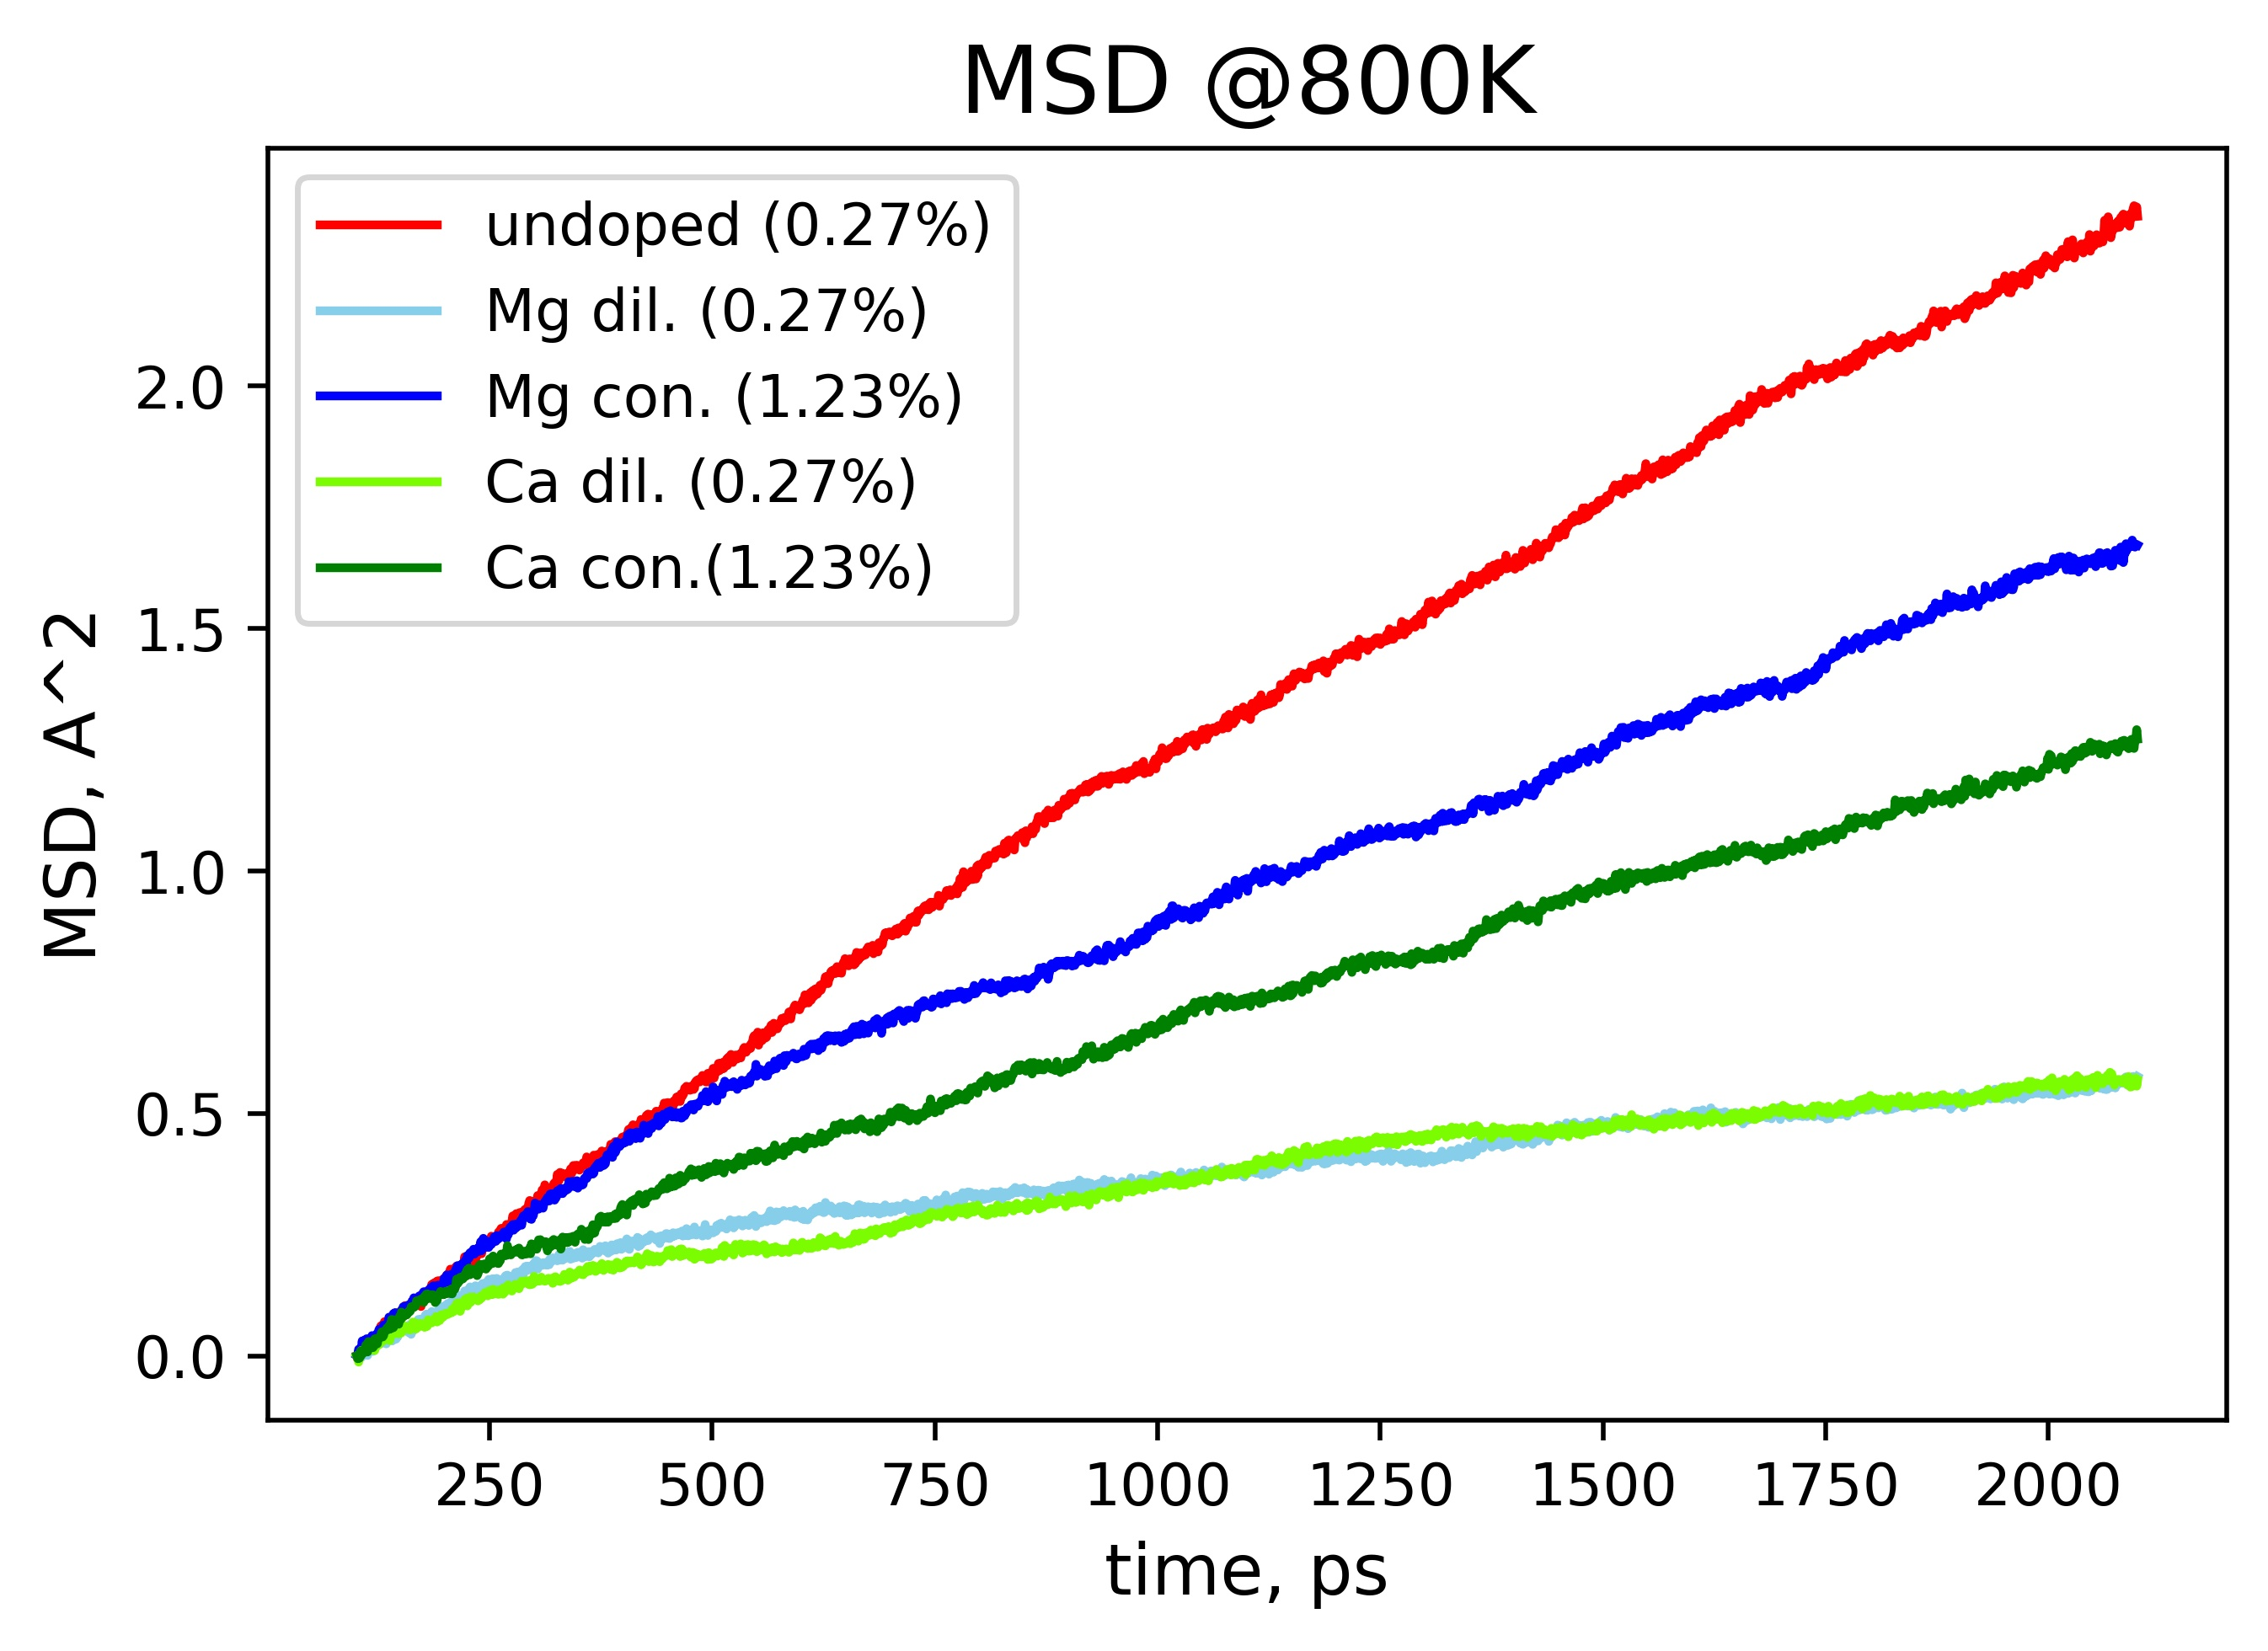
\includegraphics[width=0.45\textwidth]{800k.jpg}
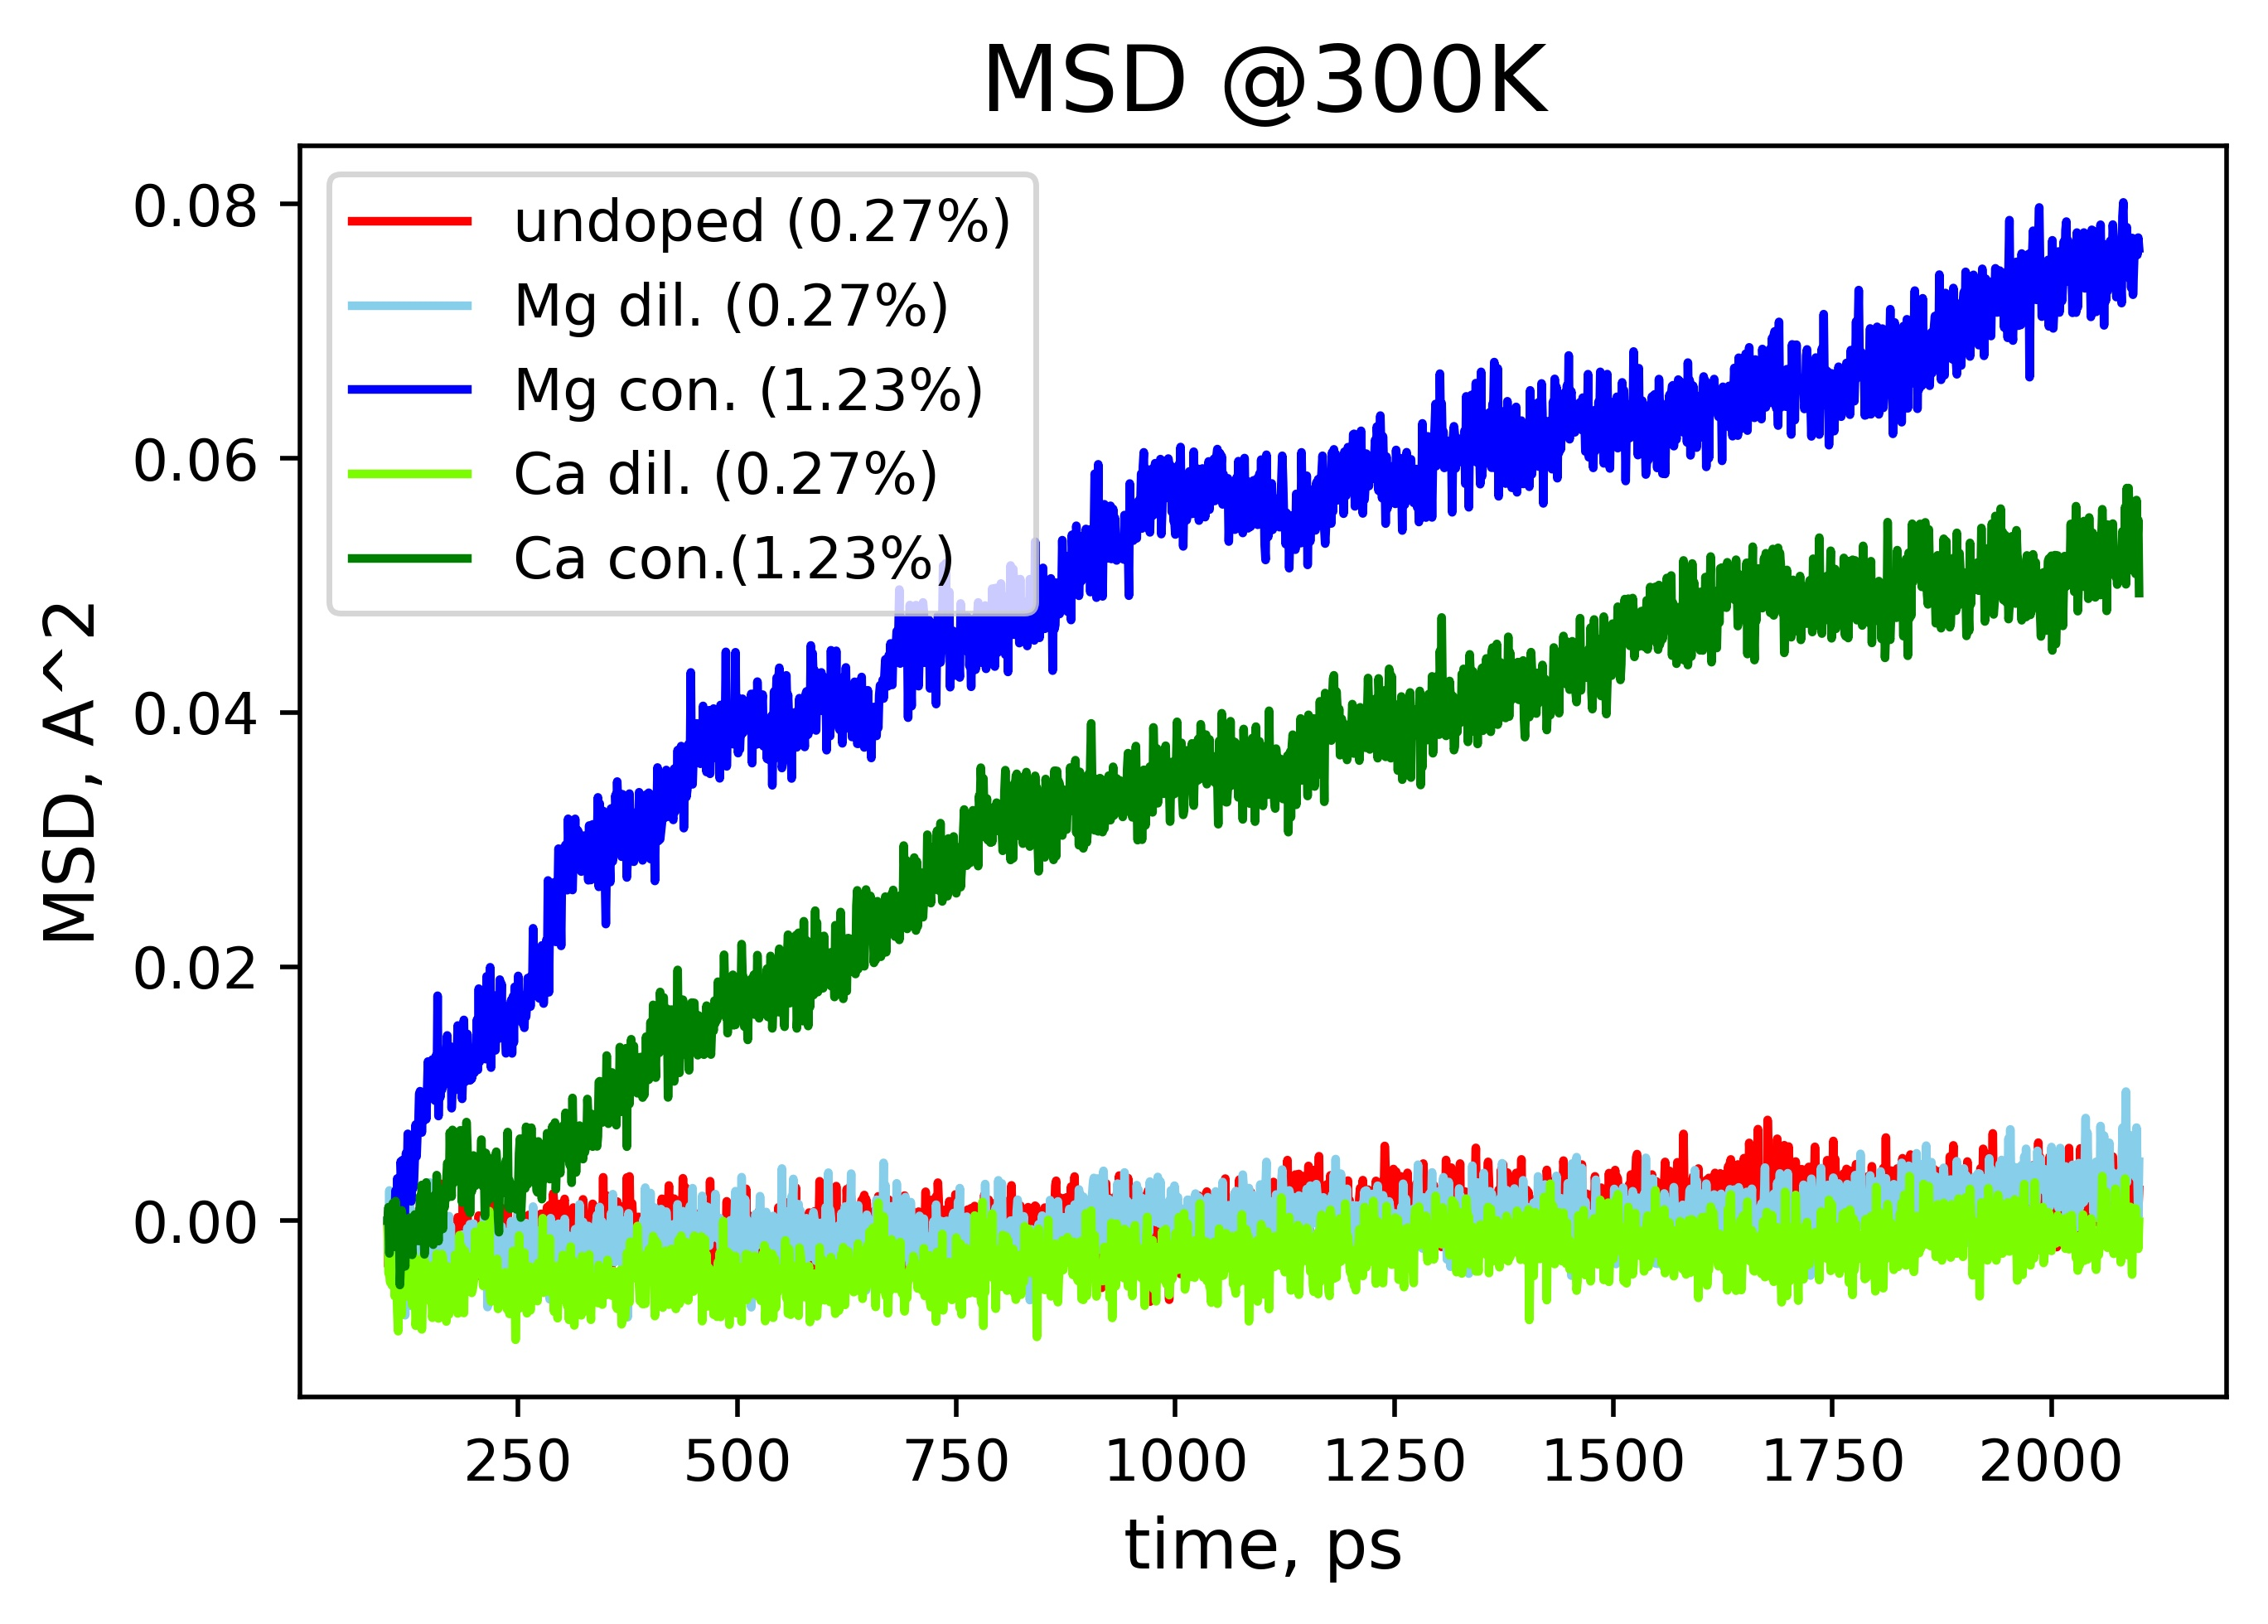
\includegraphics[width=0.45\textwidth]{300k.jpg}
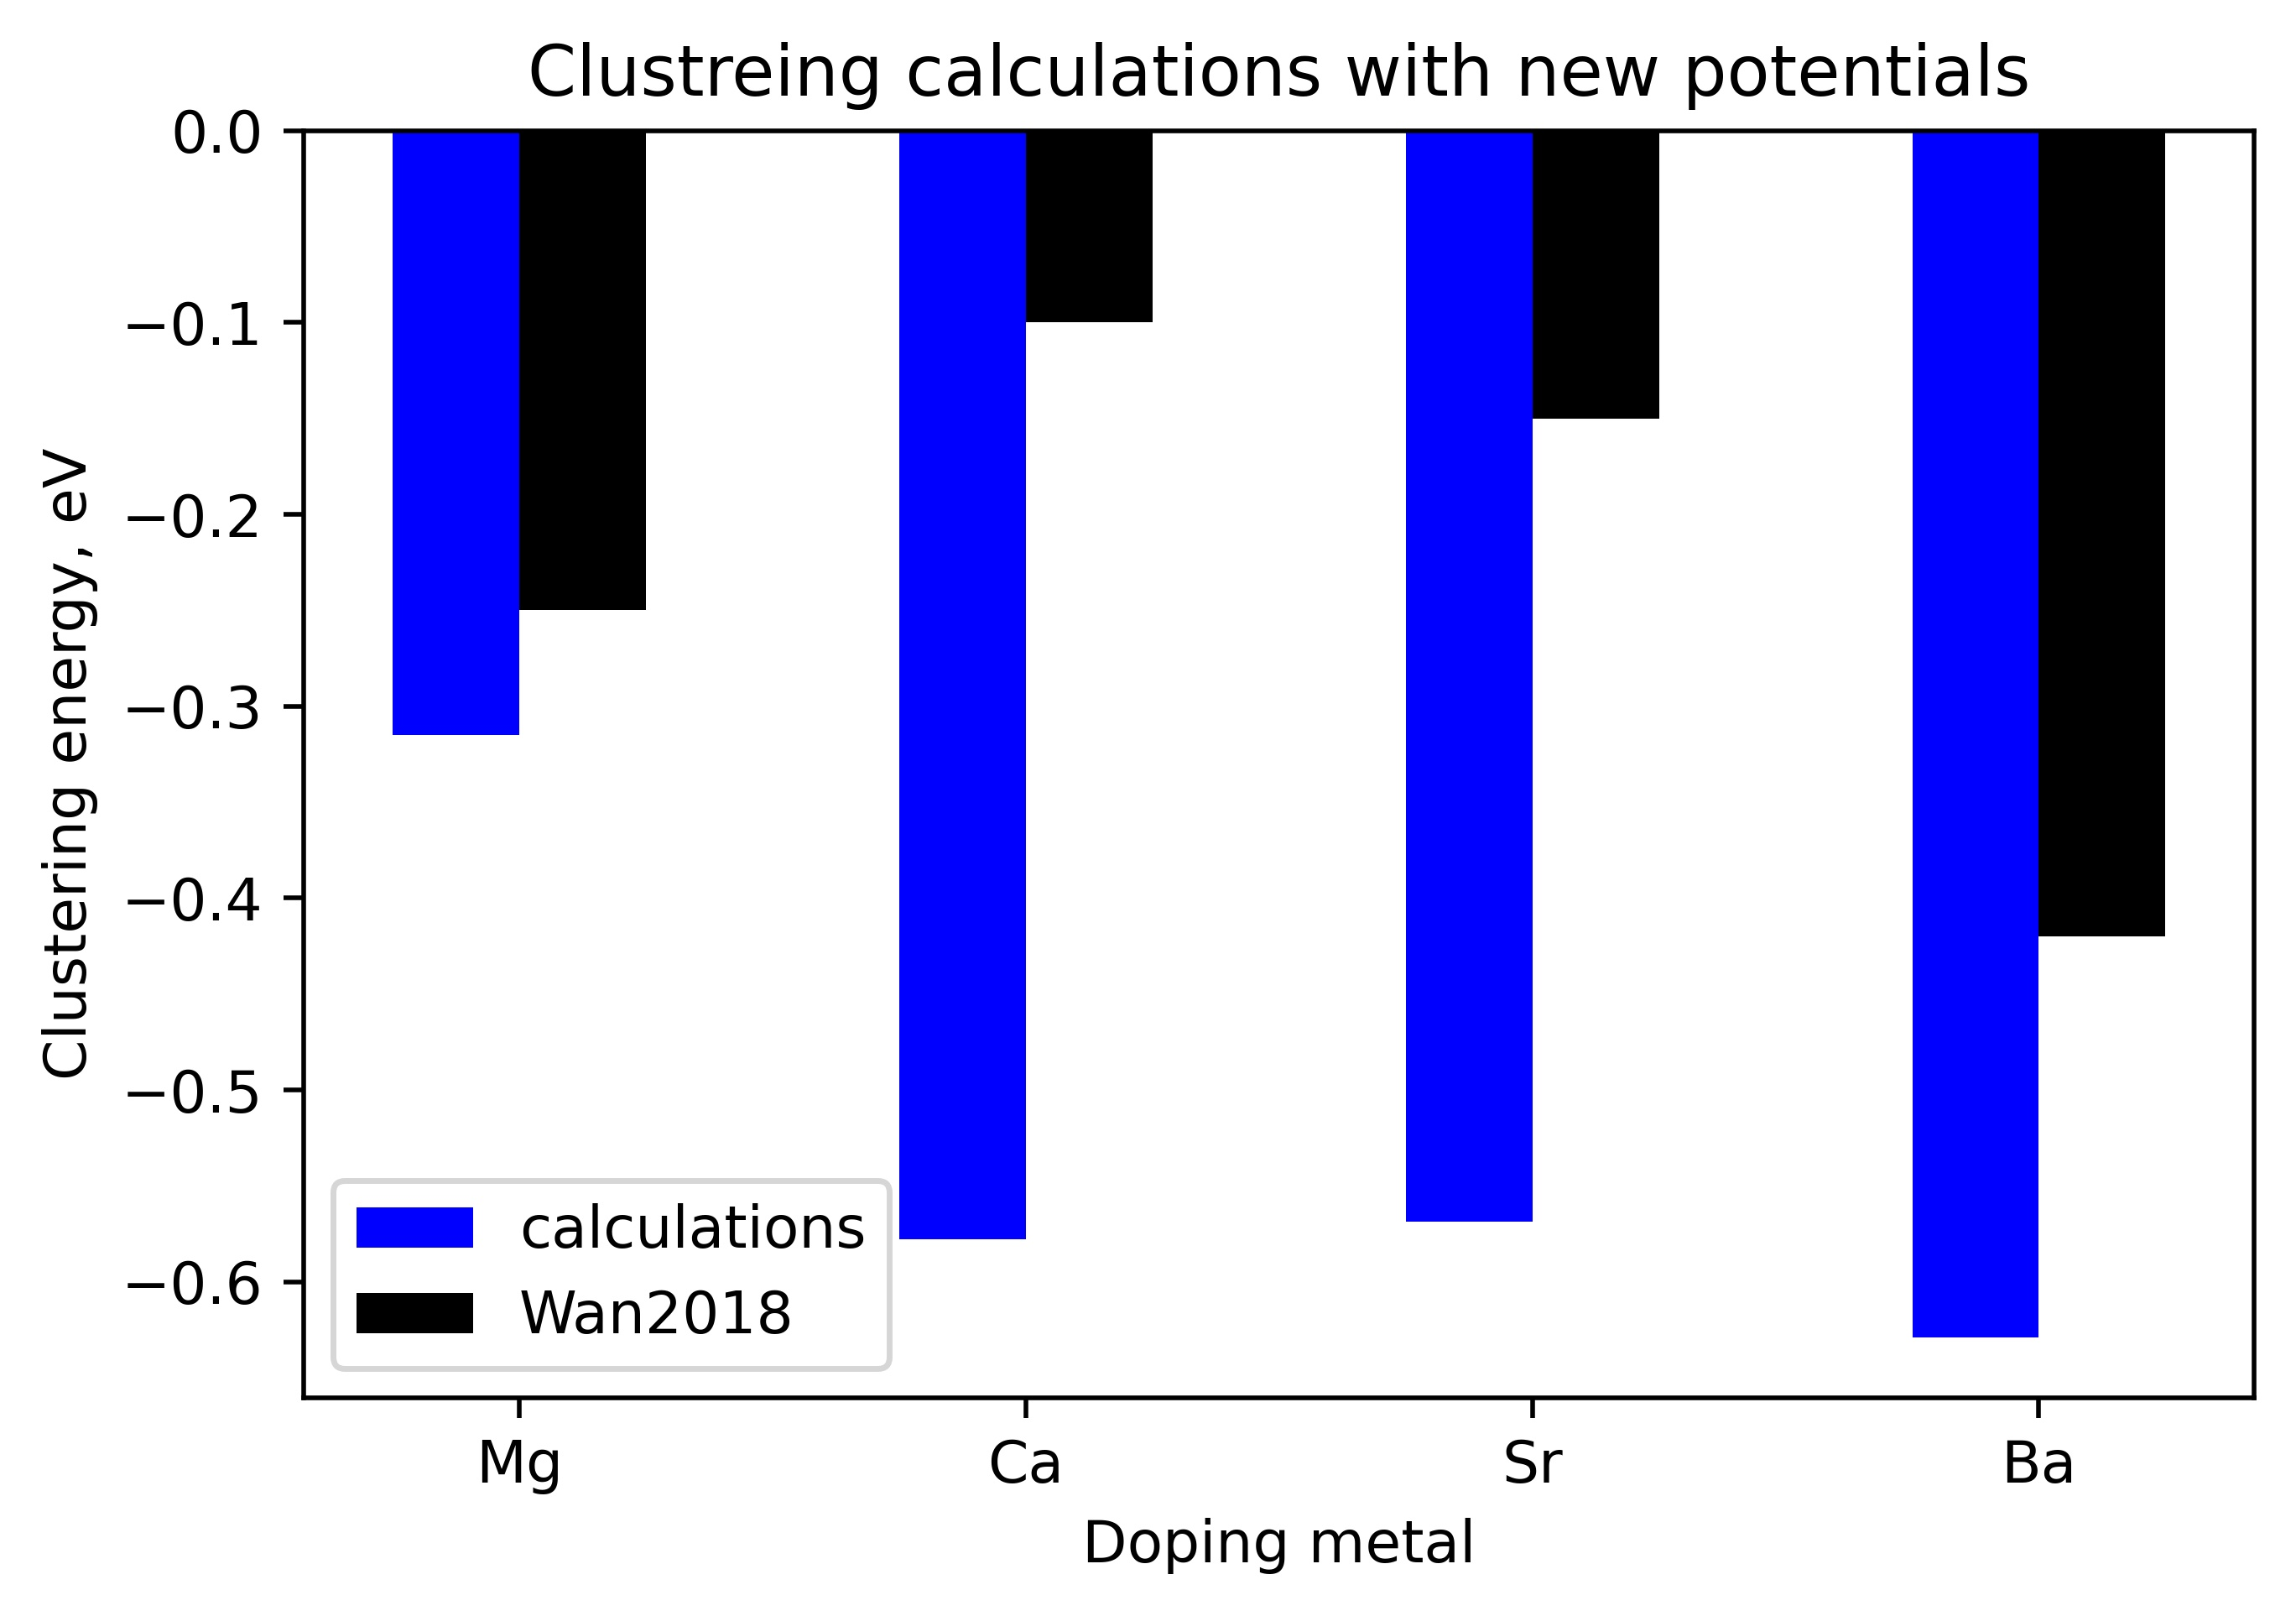
\includegraphics[width=0.45\textwidth]{clustering.jpg}
\end{figure}

\end{frame}

\begin{frame}
\frametitle{Diffusion coefficients}

\begin{table}[h!]
  \begin{center}
    \label{tab:table1}
    \begin{tabular}{l|c|c|c|c}
      \textbf{structure} & \textbf{300K, m2/s} & \textbf{800K, m2/s}\\
      \hline
      undoped & 2.68e-17 & 1.15e-14\\
      0.27\% Mg doped & 2.59e-17 & 2.26e-15\\
      1.23\% Mg doped & 2.90e-16 & 7.70e-15\\
      0.27\% Ca doped & 2.53e-17 & 2.55e-15\\
      1.23\% Ca doped & 2.68e-16 & 5.90e-15\\
    \end{tabular}
  \end{center}
\end{table}

\end{frame}

\begin{frame}
\frametitle{Halospinel modelling}

\begin{itemize}
  \item the search for Sc-Cl potential
  \begin{itemize}
    \item found a Born-Mayer potential from 2009
    \item can use these numbers after some algebraic adjustment?
  \end{itemize}
  \item structural questions
  \begin{itemize}
    \item random (these sites are all equivalent) positions of Sc in 1/3 of the spinel-like (spl) octahedral sites (1/2 of total octahedral sites are spl, so 1/6 of octahedral sites filled with Sc)
    \item random (as "Li site energies are relatively similar") positions of Li in remaining 2/3 spl octahedral sites (2/6 of tot oct), spl tetrahedral sites (1/8 of tot tet), non-spl octahedral sites (3/6 of tot oct) and non-spl tetrahedral sites (7/8 of tot tet)
    \item taking 3 unit cells: of the possible Sc sites (6) 2 occupied; after this of the possible Li sites (34) 6 occupied
    \item ASSUMPTION: Li can be in any tetrahedral hole even in those where all 4 sides are face-sharing with spl octahedra (3 of these in above example, 3 of them don't share any faces - these are the spl tetrahedrals, remaining 18 share 2 faces with spl octahedra)
  \end{itemize}
\end{itemize}

\end{frame}

\end{document}